
\documentclass[12pt]{article}
\usepackage{amsmath}
\DeclareMathOperator*{\argmin}{arg\,min} % thin space, limits underneath in displays
\DeclareMathOperator*{\argmax}{arg\,max} % thin space, limits underneath in displays
\newtheorem{thm}{Theorem}
\usepackage{amssymb}
\usepackage{amsfonts}
\usepackage{mathrsfs}
\usepackage{bm}
\usepackage{indentfirst}
\setlength{\parindent}{0em}
\usepackage[margin=1in]{geometry}
\usepackage{graphicx}
\usepackage{setspace}
\doublespacing
\usepackage[flushleft]{threeparttable}
\usepackage{booktabs,caption}
\usepackage{float}
\usepackage{graphicx}

\usepackage{import}
\usepackage{xifthen}
\usepackage{pdfpages}
\usepackage{transparent}

\newcommand{\incfig}[1]{%
\def\svgwidth{\columnwidth}
\import{./figures/}{#1.pdf_tex}
}




\usepackage{graphicx}
\usepackage{xspace,color}
\usepackage{url}
\usepackage{listings}


\lstset{commentstyle=\color{gray},keywordstyle=\color{black},
showstringspaces=false, basicstyle = \small
} %% basicstyle set fontsize
\lstnewenvironment{rc}[1][]{\lstset{language=R}}{}
\newcommand{\ri}[1]{\lstinline{#1}}  %% Short for 'R inline'



\lstdefinelanguage{language=R}{
numbers=left,
numberstyle=\footnotesize,
numbersep=1em,
xleftmargin=1em,
framextopmargin=2em,
framexbottommargin=2em,
showspaces=false,
showtabs=false,
showstringspaces=false,
frame=l,
tabsize=4,
}











\title{Something you need to know}
\author{Synferlo}
\date{May. 4, 2021}


\begin{document}
\maketitle
\newpage





\section{Sampling Distribution}

\subsection{Std. deviation vs. Std. error}
Two important parameters in each distribution: mean, standard deviation.

Given the sample data, we want to estimate the distribution of the 
population, i.e., want to know which distribution generate the data.

By estimating the distribution, we estimate the mean and the std 
deviation. The estimated std deviation of a sampling distribution is
referred to as a {\underline {std error.}}

\begin{equation*}
\text{ Std. deviation } = \sqrt {\text{ variance }}
\end{equation*}


\subsection{Estimate sampling distribution}
Mean of the sampling distribution should be the same as the true mean,
$ \mathbb{E}(\mu_{X}) = \mu $. And the std. error, $ s_{X} $:
\begin{equation*}
s_{X} = \sqrt { \frac{\text{ variance }}{n}} = 
\sqrt { \frac{\sigma^{2}}{n}} = \frac{\sigma}{\sqrt {n}}
\end{equation*}



Suppose we generate a sample, with size 5, 
from $ Normal(\mu = 22, \sigma^{2} = 1.5^{2}) $,
the standard error for the sampling distribution would be
\begin{equation*}
s_{X} = \frac{\sigma}{\sqrt {n}} = \frac{1.5}{\sqrt {5}} \approx 0.671
\end{equation*}

Then we can use R to plot the sampling and true distribution.

\begin{figure}[H]
\caption{Sampling vs. True distribution}
\center{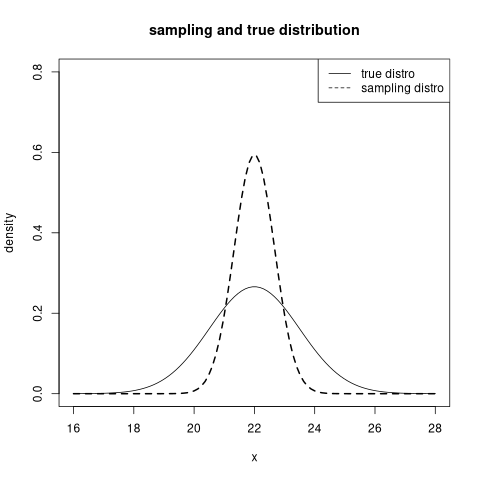
\includegraphics[scale =.5 ]  {figures/sampling_vs_true_distribution.png}}
\end{figure}


Clearly, the sampling distribution is taller and skinner, while the
true distribution is flatter.





\subsubsection{Confident Interval for the mean}

By doing this, must assume the data is normally distributed.

Then,

Step 1: Compute sample mean, $ \mu_{X} $ and std deviation, $ s_{X}$. 
(page 394 in Tilman's R code book)

Step 2: Compute sample std. error. 
\begin{equation*}
		se = \frac{s_{X}}{\sqrt {n}}
\end{equation*}


Step 3: Since we assume obs are normally distributed and we are using
$ s_{X} $ rather $ \sigma_{X} $, t-distribution with $ n - 1 $ degree
of freedom is the appropriate method, where $ n $ is the sample size.


Step 4: Choose the confident interval, e.g., 95\% . It says 
$ \alpha = 0.05 $. Hence the {\underline {critical value}} is 
\begin{equation*}
\text{ cumulative probability } = 1 - \frac{\alpha}{2} = 0.975
\end{equation*}
Now we have the cumulative probability, p, for the qt() function in R.
We can use the following code to compute the critical value (or called
the quantile value in R).

\noindent\fbox{%
\parbox{\textwidth}{%

$ \alpha $ = 0.975\\
\#You need to substitute n by the actual sample size.\\
critical\_value  = qt(p = $ \alpha $, df = n - 1) \\
print(critical\_value)\\
\#it is the value on the horizontal axis, if you plot the density
of t-distribution.

}%
}\\

So the area within the confidence interval(CI) is $ prob. = .95 $

\begin{figure}[H]
		\center{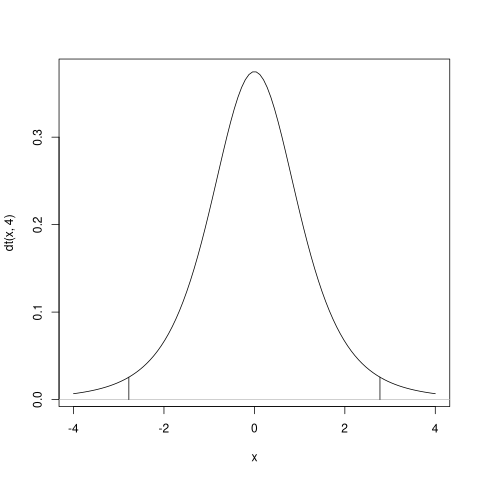
\includegraphics[scale = 0.5 ]  {figures/confidence_interval.png}}
\end{figure}


Step 5: Now you have sample mean ($ \mu_{X} $), std error ($ se $), 
and the critical value for .95 confidence interval. Then you can 
make the following inference:

\noindent\fbox{%
\parbox{\textwidth}{%

I am in 95\% confidence saying that the true mean of the population
lies somewhere between
\begin{equation*}
\mu_{X} - se  \times \text{ critical\_value } <
\quad \mu \quad < \mu_{X}  + se  \times \text{ critical\_value }
\end{equation*}
}%
}\\






\section{Hypothesis Test}
\subsection{null and alternative hypothesis}
\subsubsection{Null Hypo.}
Null Hypothesis: $ H_0 $. The claim that is assumed to be true.

\subsubsection{Alt. Hypo.}
All. hypo.: $ H_1 $. The conjecture that you are testing for, against
the null.

Three types of tests based on different $ H_1 $:

1. lower-tailed test: When $ H_1 $ is defined in terms of a less-than
statement, with $ < $. It is {\underline {one-sided}}.

2. upper-tailed test: When $ H_1 $ is defined in terms of a greater-than
statement, with $ > $. It is {\underline {one-sided}}.

3. two-tailed test: When $ H_1 $ is defined in terms of a different-to
statement, with $ \ne $. It is {\underline {two-sided}}.










\subsection{Test statistics}

The statistic that is compared to the appropriate standardized
sampling distribution to yield the $ p $-value.


\subsection{$ p $-value}

The meaning for $ p $-value in different types of test:

1. In a lower-tailed test: $ p $-value is a left-hand tail probability
from the sampling distribution of interest.

2. In an upper-tailed test: a right-hand tail prob. 

3. In two-sided test, the sum of left and right tail probability.
This is equivalent to two times the area in one tail when the
sampling distribution is {\underline {symmetric}}.\\




Consider and example:


\begin{figure}[H]
		\center{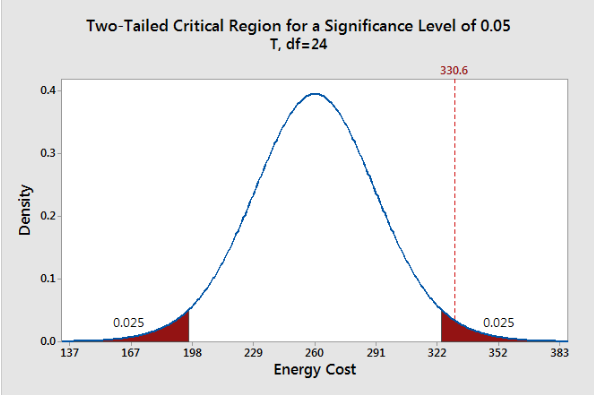
\includegraphics[scale =.5 ]  {figures/CI_95.png}}
		{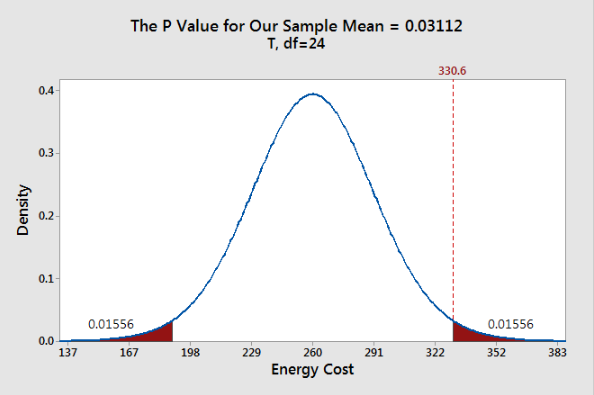
\includegraphics[scale =.5 ]  {figures/pvalue_against_CI.png}}
\end{figure}

$ H_0 $: the population mean is 260\\
$ H_1 $: the population mean differs from 260

After calculation, we get the sample mean is $ 330.6 $

Red area in the left figure stands for the area of our 95\% CI.
Clearly, our sample mean is outside the CI.

Red area in the right figure stands for the $ p $-value for this sample
mean. Note, we can compute this by using pnorm() in R.
The $ p $-value says the prob. of obtaining a {\underline {sample mean}}
that is as extreme (or even far away from the true mean, 260) as what
we got (330.6) is $ 0.01556  \times 2 = 0.03112 $.


Clearly, when the sample mean appears outside the 95\% CI, the
$ p $-value is also less than the significance level, 
$ 0.03112 < 0.05 $. Or we say 
{\underline {$ p $-value is less than the significance level}}.


Since our sample mean is outside the 95 CI, we CANNOT say that
the population mean is 260 with 95\% confidence. That's why we 
{\underline {reject the null when $ p $-value $ < $ the 
significance level.}}


Remember, $ p $-value is calculated based on the position of your
sample mean. If the $ p $-value is less than the significance level, 
{\underline {your sample mean is outside the CI}}. Hence, we 
reject the null.


\subsection{Comments on Hypothesis Test}

1. $ p $-value never provides ``proof" of either $ H_0 $ or $ H_1 $ being
{\underline {truly}} correct.

Rejecting $ H_0 $ merely implies that {\underline {the sample data
suggest $ H_1 $ ought to be preferred.}}\\










\subsection{Testing Means (single mean)}

How to test the mean with t-test? Let's do this.


Suppose you have a sample from the population with mean = 80. You
want to test if the true mean, i.e., population mean, is 80 with 95
confidence.

\begin{align*}
H_0: \mu &= 80\\
H_1: \mu &\le 80
\end{align*}



By doing this, we need to:

step 1: compute sample mean($  \overline{X} $) and the sample std 
deviation, or SD in short ($ s $).\\
mean = $ 80.10174 $, SD = $ s $ = $ 1.651756 $.
\\

step 2: compute test statistic T:
\begin{equation*}
T = \frac{ \overline{X} - \mu}{s/\sqrt {n}} \approx 0.3895706
\end{equation*}	
The dashed line stands for t = 0.3895706.
Note, the sample SD, $ s/\sqrt {n} $, is the estimated standard 
error of the mean.

T follows a t-distribution with $ n - 1 $ degree of freedom.\\

step 3: Note, $ H_1 $ suggests that this is a left-tailed test. So,
the $ p $-value is provided as the area under the sampling distribution
(a t-distribution with DOF = 39) to the left of a vertical line at T.

Now, compute the $ p $-value = $ 0.6505133 $. It says the area at the
left side of the dashed line is about 0.65 (The cumulative prob.).


step 4: Compare the $ p $-value with significance level, $ \alpha $.
Clearly, $ p $-value is much greater than 0.05. 
{\underline {We fail to reject the null}}. It pretty much makes sense
because the sample we use is generated from a normal distribution with
mean = 80. It is very unlikely we can reject the null. The code is 
below.

\begin{figure}[H]
		\center{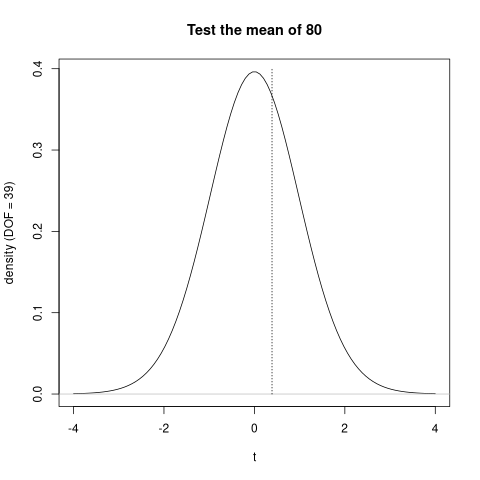
\includegraphics[scale =.5 ]  {figures/t-test.png}}
\end{figure}









\begin{rc}
 
# generate a sample
n = 40
# make sure we have the same generated numbers, set the seed
set.seed(5)
sample = rnorm(n, 80, 1.5)
# compute the sample mean and SD
sample_mean = mean(sample)			# X = [1] 80.10174
# sample SD: s
sample_sd = sd(sample)				# s = [1] 1.651756
sample_se = sample_sd/sqrt(n)	# [1] 0.2611655

# T statistics:
sample_T = (sample_mean - 80)/sample_se		# [1] 0.3895706

# compute the p-value, i.e., the cumulative prob. using pt()
# remember, sample_T is t value on the horizontal axis of the density.
sample_p_value = pt(sample_T, n-1)		# [1] 0.6505133

# Clearly, p-value is much greater than 0.05. We fail to reject 
# the null.


# Method 2
# R has a built in function for t-test:
# t.test(x = sample, mu = mean, alternative = '')
# alternative can be two.sided, less, greater


t.test(x = sample, mu = 80, alternative = 'less')

#	        One Sample t-test
#	
#	data:  sample
#	t = 0.38957, df = 39, p-value = 0.6505
#	alternative hypothesis: true mean is less than 80
#	95 percent confidence interval:
#	     -Inf 80.54177
#	sample estimates:
#	mean of x
#	 80.10174

\end{rc}











\subsection{Testing Means (two mean)}


Sometime, testing for one mean is not enough. You may want to compare
the means of two distinct groups of measurements, which boils down
to a hypothesis test for the true difference between two means, 
$ \mu_1, \mu_2 $.


Two groups of data relate to each other affects the specific form of
standard error for the difference between two sample means and 
therefore the test statistics itself. 
Normally, $ H_0 $ would be $ \mu_1 = \mu_2 $.\\

Case 1:\\
When you cannot assume the {\underline {variances}} of the two 
populations are {\underline {equal}}, then you perform the 
{\underline {unpooled}} version of the two-sample t-test.\\

Case 2:\\
If you can safely assume {\underline {equal variances}}, then you
can perform a {\underline {pooled}} two-sample t-test, which
{\underline {improve the precision of the result}}.



\subsubsection{Unpooled two-sample t-test}

Suppose we have two samples from $ N(76, 2) $, $ N(80, 2) $, with size
$ n_1 = 44 $, $ n_2 = 31 $. Clearly, we manually make the population
of these two samples
with $ \mu_1 = 76 $, $ \mu_2 = 80 $. Now let's use t-test to verify
the following null hypothesis. (Note, we are testing the mean of the
population.)
\begin{align*}
H_0:& \mu_1 - \mu_2 = 0\\
H_1:& \mu_1 - \mu_2 < 0
\end{align*}


We can use Welch's t-test:

Form the $ t $ ststistics for two-sample case,
\begin{equation*}
T = \frac{\mu_{X_1} - \mu_{X_2} - \mu_0}{\sqrt {
		\frac{s_1^{2}}{n_1} + \frac{s_2^{2}}{n_2}
}}
\end{equation*}

where $ \mu_0 $ is the null value of the interest, which is
$ \mu_0 = \mu_1 - \mu_2 = 0 $.

And this $ t $ statistic is approximately following a t-distribution
with $ df $ degree of freedom, where
\begin{equation*}
df = \left[ 
		\frac{(\frac{s_1^{2}}{n_1} + \frac{s_2^{2}}{n_2})^{2}}
		{ \frac{(\frac{s_1^{2}}{n_1})^{2} }{n_1 - 1} + 
		\frac{ (\frac{s_2^{2}}{n_2} )^{2} }{n_2 - 1}
		}
\right] 
\end{equation*}

The above equation for $ df $ is called the {\underline {
				Welch-Satterthwaite equation.
}}



\noindent\fbox{%
\parbox{\textwidth}{%
Note, the numerator of $ T $ should be consistent with the hypothesis.
Here, we are testing for either $ \mu_1 - \mu_2 = 0 $ or 
$ \mu_1 - \mu_2 < 0 $, so in $ T $ we write 
$ \mu_{X_1} - \mu_{X_2} $. It is a lower-tailed test

If you write your hypothesis in this way,
\begin{align*}
H_0:& \mu_1 - \mu_2 = 0\\
H_1:& \mu_1 - \mu_2 > 0.
\end{align*}

Then it will be a upper-tailed test. And you want to check to right
tail, rather the left one .

}%
}\\


In method 1, I compute the $ t $ statistics and $ p $-value by
myself. $ T = -299.4002 $, $ p $-value = 2.560795e-107.
It is clearly less than 99\% confidence interval. Hence, we can reject
the null. It says that the population means are not likely to be equal
based on our sample.

You can check the figure below. At left tail, the probability is 
almost zero even when $ t $ is around 4. Hence, out $ t = -299 $ must
be closed to 0. And this is verified by the $ p $-value.


\begin{figure}[H]
		\center{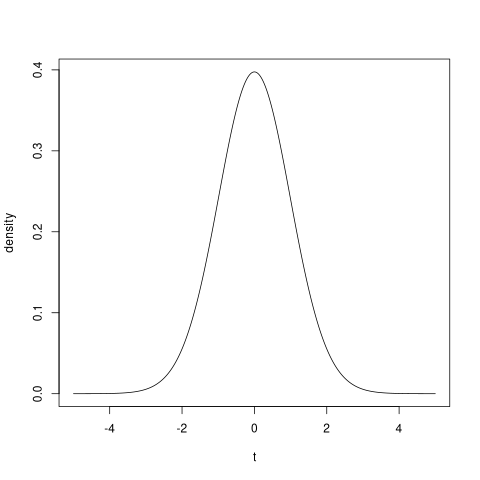
\includegraphics[scale =.5 ]  {figures/t-test_two_mean.png}}
\end{figure}



Instead of writing the code by myself, R also have a built-in function
for Welch's t-test.


\begin{rc}

# Method 1
# Generate data from N(76,2), N(80,2)
set.seed(5)
n1 = 44
n2 = 31
sample1 = rnorm(n1, 76, 2)
sample2 = rnorm(n2, 80, 2)


# Compute sample mean and se, i.e., s
sample1.mean = mean(sample1)		# [1] 76.24008
sample2.mean = mean(sample2)		# [1] 79.66198


sample1.s = sd(sample1)/n1			# [1] 0.05069484
sample2.s = sd(sample2)/n2			# [1] 0.04731536


# Compute df:

df.upper = ((sample1.s**2/n1) + (sample2.s**2/n2)) ** 2
df.lower.left = (sample1.s**2/n1)**2/(n1-1)
df.lower.right = (sample2.s**2/n2)**2/(n2-1)
df.lower = df.lower.left + df.lower.right

df = df.upper/df.lower				# [1] 67.39422


# Compute t statistics
t.upper = sample1.mean - sample2.mean
t.lower = sqrt(
		(sample1.s**2/n1) + (sample2.s**2/n2)
)
# It is negative because we are doing a left-tailed test.
sample.t = t.upper/t.lower		# [1] -299.4002

# p-value
pt(sample.t, df)			# [1] 2.560795e-107

# Suppose we use 99 Confidence Interval, p-value here is clearly
# less than 0.01
# Great, we reject the null. Hence miu_1 < miu_2. It is being verified.


png('figures/t-test_two_mean.png')
x = seq(-5,5, length = 2000)
plot(x,
		 dt(x, df),
		 type = 'l',
		 xlab = 't',
		 ylab = 'density'
)
dev.off()


# Method 2
# Built-in Welch's t-test
t.test(x = sample1, y = sample2, alternative = 'less', conf.level = 0.99)



#	        Welch Two Sample t-test
#	
#	data:  sample1 and sample2
#	t = -8.0105, df = 72.718, p-value = 6.891e-12
#	alternative hypothesis: true difference in means is less than 0
#	99 percent confidence interval:
#	      -Inf -2.405759
#	sample estimates:
#	mean of x mean of y
#	 76.24008  79.66198
\end{rc}










\subsection{Testing Categorical Variables}

We use $ Z $-test to conduct a proportion test,
see chapter 18.3(Tilman). Z-test is a normal-based test (normal distri).
It is to data that are binary in nature.

To test {\underline {categorical variables}} with more than two
distinct level, we use {\underline {Chi-square test}}, or called
$ \chi^{2} $ test.\\


Two common variants of $ \chi^{2} $ test: 

1. Goodness of fit(GOF) test, a $ \chi^{2} $ test of distribution.
It is used when assessing the frequencies in the levels of a 
{\underline {single}} categorical variable(CV).(You only have one CV)


2. Test of independence. Employed when you have two CV.




\subsubsection{Single Categorical Variable}
Goal:

You want to find out what proportion of n obs fall into each defined
category.\\

Assumption: categories are mutually exclusive and exhaustive.

\noindent\fbox{%
\parbox{\textwidth}{%
Mutually exclusive:\\
obs cannot take more than one of the possible categories. For example,
A take Math class, then it cannot take another English class.\\

Exhaustive:\\
Categories cover all possible outcomes.


}%
}\\


Suppose we want to test if the observations uniformly fall in three
categories, 
\begin{align*}
		H_0&: \pi_{0(1)} = \pi_{0(2)} = \pi_{0(3)} = \frac{1}{3}\\
		H_1&: H_0 \text{ is incorrect. }
\end{align*}





Define:

1. n: number of obs\\
2. k: number of categories(levels) for the CV.\\
3. $ \pi_{i}$, where $ i = 1, ..., k $: the proportion of n obs in each
of k categories.\\
\noindent\fbox{%
\parbox{\textwidth}{%
Example:\\
You have 100 obs fill in 3 categories (levels) of A, B, and C.
Then, the proportion of n obs in each categories would be
\begin{align*}
		\pi_{A} = \frac{a}{n},\quad \pi_{B} &= \frac{b}{n}, \quad
		\pi_{C} = \frac{c}{n}\\
		\quad a + b + c &= n = 100
\end{align*}
}%
}\\


4. $ \pi_{0(i)} $: the assumed proportion of n obs in each category
in the null hypothesis. Subscript $ 0 $ stands for the null.\\
5. $ O_{i} $: number of the obs from the data fall in the $ i $th 
category. In the above example, $ O_{A} = a, O_{B} = b, ... $.\\
6. $ E_{i} $: the expected count(null) in the $ i $th category, i.e, 
$ E_{i} = n  \times \pi_{0(i)} = n  \times \frac{1}{3} $.\\


Now, we can form the $ \chi^{2} $ statistics:
\begin{equation*}
\chi^{2} = \sum\limits_{i = 1} ^k
\frac{(O_{i} - E_{i})^{2}}{E_{i}}
\end{equation*}

Statistics $ \chi^{2} $ follows a Chi-square distribution with
$ df = k - 1 $ degree of freedom.\\

\newpage
\noindent\fbox{%
\parbox{\textwidth}{%

Something you NEED to know about the $ \chi^{2} $ test.

1. Goodness of fit(GOF): the proximity of the data to the distribution
hypothesized in $ H_0 $.

2. {\underline {Positive}} extremity of the $ \chi^{2} $ 
statistics provides evidence {\underline {against}} $ H_0 $.
So, $ p $-value is {\underline {always}} computed as an 
{\underline {upper-tail area}}.

3. A {\underline {rejected $ H_0 $}} DOES NOT tell you about the 
true values of $ \pi_{i} $. It merely suggests that they do not follow
$ H_0 $ specifically.




}%
}\\


The $ \chi^{2} $ distribution with different degree of freedom(DOF),

\begin{figure}[H]
		\center{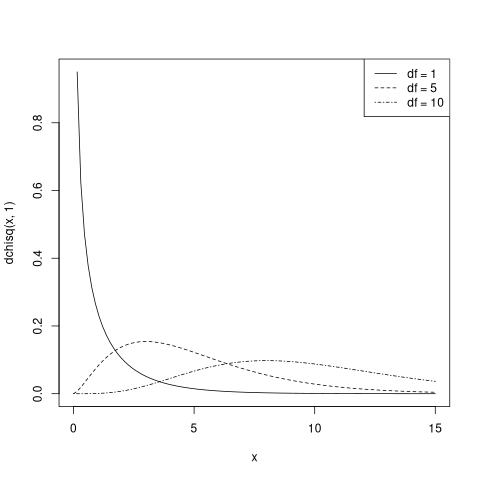
\includegraphics[scale =.5 ]  {figures/Chi-square_1_5_10.png}}
\end{figure}


Because it is unidirectional, the $ p $-value being defined as
{\underline {upper-tail areas ONLY.}}


We can run this test by either compute the test statistics by ourselves,
or use the built-in function for $ \chi^{2} $ test.
Notice, the built-in function chisq.test() requires the
{\underline {frequencies}} of the data. DO NOT pass the raw data
into this test. Code :

\begin{rc}

### Method 1: Write your own chi-square test

## test example:

# Suppose data fall in three categories, 1,2,3.
# step 1: generate data

sample = c(2,3,2,3,2,1,3,3,2,2,3,2,2,2,3,3,3,2,3,2,
2,2,1,3,2,2,2,1,2,2,3,2,2,2,2,1,2,1,1,1,2,2,2,3,1,2,1,2,1,2,1,3,3)

n = length(sample)		# [1] 53

# step 2: compute O_i
sample.table = table(sample)
sample.table
#		sample
#		 1  2  3	-> category i
#		11 28 14	-> O_i

# We can also comute the actual pai_i by dividing sample.table by n
# but we don't need to to form the test statistics
pai_i = sample.table/n
pai_i
#	        1         2         3		-> i
#	0.2075472 0.5283019 0.2641509		-> pai_i

# step 3: compute pai_0(i), the expected proportion,
pai_i_expected = (1/3)*n		# [1] 17.66667


# step 4: compute test statistics kai^2

kai_sq = sum((sample.table - pai_i_expected)**2/pai_i_expected)	
# kai_sq = 9.320755


# step 5: compute p-value
# Note, pchisq() give the cumulative prob. from CDF. We need to
# subtract it by 1 to get the area for right tail.

df = 3-1
p_value = 1 - pchisq(kai_sq, df)		#[1] 0.009462891

# Clearly, it is less than 0.001 significant level. We can reject the
# null. The data do not suggest that the proportions of each category
# are same.
# We can also check it by printing out the proportion, pai_i
sample.table/n
#	        1         2         3
#	0.2075472 0.5283019 0.2641509

# Clearly, not the same.


# Now plot the density

x = seq(0,15, length = 100)
png('figures/single_categorical_chisq_test.png')
plot(
		 x,
		 dchisq(x, 3),
		 type = 'l',
		 xlab = 'Chi-square',
		 ylab = 'density(df = 2)',
		 main = 'Chi-square test for single categorical variable'
)
abline(h = c(0), col = 'gray')
abline(v = c(kai_sq), col = 'gray')
dev.off()





### Method 2:
# R has a built-in function for chi-square test.


# NOTICE: this test function require the vector of
#	the obs Frequencies! 
# DO NOT pass raw sample into it.

chisq.test(x = sample.table)

#	        Chi-squared test for given probabilities
#	
#	data:  sample.table
#	X-squared = 9.3208, df = 2, p-value = 0.009463



\end{rc}




Up to now, we assume the proportion of different categories are 
uniformly distributed. What if it is not?
Suppose, we want to test if the proportions of the aboved sample 
is $ \pi_1 = 0.25, \pi_2 = 0.5, \pi_3 = 0.25 $, then we need
to specify $ p $ in $ chisq.test(x = , q = ) $.
\begin{align*}
H_0&: \pi_{0(1)} = 0.25, \pi_{0(2)} = 0.5, \pi_{0(3)} = 0.25\\
H_1&: H_0 \text{ is incorrect. }
\end{align*}

Code:
\begin{rc}
chisq.test(x = sample.table, p = c(0.25, 0.5, 0.25))
#        Chi-squared test for given probabilities
#
#data:  sample.table
#X-squared = 0.50943, df = 2, p-value = 0.7751

# Now, we cannot reject the null
\end{rc}




\subsubsection{Two Categorical Variables}

Categorical variable A and B are mutually exclusive and exhaustive.\\
Our goal: test if A and B are related/dependent, i.e, check if the 
distribution of frequencies change together. If they are independent,
distribution of frequencies in A will have nothing to do with B's.

This is also call {\underline {a test of independent }}

\begin{align*}
H_0&: \text{ A and B are independent. }\\
H_1&: \text{ A and B are dependent }
\end{align*}

Consider an example:

Two categorical variables: 1) Treatment Method, and 2) Effect.

Levels in Treatment Method: Injection, Tablet, Laser, Herbal.

Levels in Effect: None, Partial, Full


Compute $ chi^{2} $ statistics
\begin{equation*}
		\chi^{2} = \sum\limits_{i = 1} ^{k_{r}} \sum\limits_{j = 1} ^{k_{c}}
\frac{
		(O_{i,j} - E_{i,j})^{2}}{ E_{i,j}}
\end{equation*}

$ k_{c} $: the column level of the variable, here
we have three columns, $ k_{c} = 3 $.\\
$ k_{r} $: the row level of the variable, $ k_{r} = 4 $.\\
$ O_{i,j} $: the observed count\\
$ E_{i,j} $: the expecred count
\begin{equation*}
E_{i,j} = \frac{
		\left( 
				\sum\limits_{u = 1} ^{k_{r}} O_{u,j}	 
		\right)  \times 
		\left( 
				\sum\limits_{v = 1} ^{k_{c}} O_{i,v}
		\right) 
}
{N}
\end{equation*}

Degree of freedom: $ df = (k_{r} - 1) \times (k_{c} - 1) $\\


\noindent\fbox{%
\parbox{\textwidth}{%
{\textbf {NOTE:}}\\
1. it is NOT necessary to assume that $ k_{r} = k_{c} $.\\
2. A rejected $ H_0 $ does not tell you about the nature of how
the frequencies depend on one another.

}%
}\\

Code
\begin{rc}
chisq.test(x = sample)

#	        Pearson's Chi-squared test
#	data:  sample
#	X-squared = 66.166, df = 6, p-value = 2.492e-12
\end{rc}







\section{Hypothesis Test Errors and Power}

\subsection{The Errors}

1. Type I error:\\
The null, $ H_0 $, is true, but you reject it. The probability of 
committing such an error is equivalent to the significance level 
$ \alpha $.\\

2. Type II error:\\
You incorrectly retain a false $ H_0 $, i.e., fail to accept a true
$ H_1 $. The probability of this type of error is usually unknown since
it depends on what the true $ H_1 $ is.


The distribution, mean, and variance can affect the probability
of a type II error. 

\begin{figure}[H]
		\center{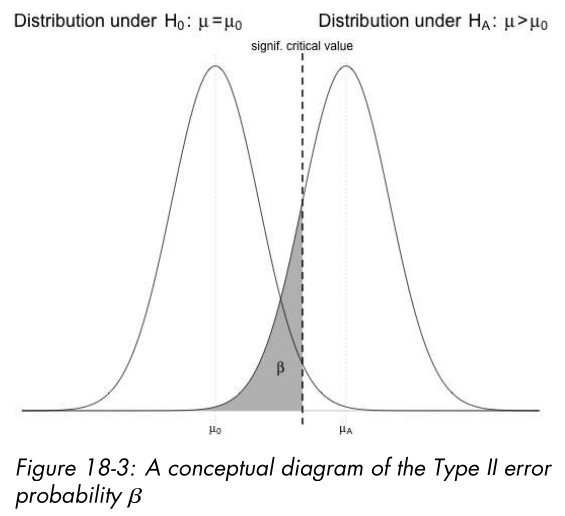
\includegraphics[scale =.6 ]  {figures/prob_of_type_II_error.png}}
\end{figure}



The distribution on the right is the true distribution specified by
$ H_1 $. The probability of the type II error (you retain a false
null) is $ \beta $.


If the true mean (from the distribution on the right) is far more
greater than the null's, then $ \beta $ would be very small.

If the variance of the true distribution is larger, the density
would be flatter, so $ \beta $ would be greater.



\subsection{The statistical power}

The $ power $ is the prob. of correctly rejecting a null that is 
unture.

For a Type II error, the statistical power is $ 1 - \beta $.




\section{Analysis of variance (ANOVA)}
DEF:\\
ANOVA is used to compare {\underline {multiple means}} in a test
for equivalence. It is a extension of the hypothesis test comparing
two mean.



\subsection{One-way ANOVA}

It is used to test {\underline {two or more}} means for equality.
It is often used to analyze experimental data to assess the impact
of an intervention.

Suppose we have $ k $ distinct groups of obs. The hypothesis would be
\begin{align*}
H_0:&\quad \mu_1 = \mu_2 = ... = \mu_{k}\\
H_1:&\quad \mu_1, \mu_2, ..., \text{ are not all equal(at least one
mean differs.). }
\end{align*}

When $ k = 2 $, the two-sample $ t $-test is equivalent to ANOVA.

{\underline {Assumptions:}}\\
ANVOA requires samples are independence, normally distributed (or
approximately so), and the variance of the {\underline {observations}}
in each group should be equal, or at least approximately so.

1. Violation of these assumptions does not mean your results will be 
worthless, but it will impact the overall effectiveness of detecting
a {\underline {true}} difference in the means.

2. The number of obs in each group does not need to be equivalent.
But it does render the test more sensitive to potentially
detrimental (negative) effects if your assumptions of equality of
variances and normality are not sound.\\



Stop here, Chapter 19.1
Switch to Linear Regression.



































\end{document}

